\documentclass[a4paper,10pt,notitlepage]{article}
\usepackage{sprawozdanie-ato}


\begin{document}


\title{\
Laboratorium Sieci Komputerowych\\\
Konfiguracja zapory sieciowej
}
\author{\
Tomasz Cudziło, Barnaba Turek\\
\textsc{PW EE Informatyka}\\[6pt]
}
\date{\today}

\maketitle
\tableofcontents


\section{Cel ćwiczenia}

W ramach laboratorium skonfigurowano zaporę sieciową do blokady określonych
typów transmisji.

W pierwszej części blokowano ruch \ssh{} pochodzący z maszyny \volt{} na
dodatkowym interfejsie. Blokadę wykonano korzystając z \pf, następnie z \ipfw,
podając reguły w trybie bezstanowym. W drugiej części wykorzytano reguły stanowe
do wykonania blokady zezwalającej na wykonanie połączenia \ssh{} zza zapory,
jednocześnie odrzucając połączenia przychodzą z zewnątrz zapory.


\section{Wstęp}
\label{sec:wstep}
\subsection{Teoria}

Zapory sieciowe to narzędzia software'owe lub hardware'owe służące ochronie
pewnego wydzielonego obszaru sieci. Umieszcza się je pomiędzy siecią wewnętrzną,
która ma podlegać ochronie, a siecią zewnętrzną, z której spodziewamy się ataków.

Zapory dzielimy na filtrujące pakiety (\ang{packet-filtering firewall}) i
pośredniczące (\ang{proxy-firewall}) \cite{wstep:stevens}. Ćwiczenie obejmuje
tylko zapory pierwszego typu.

Zapory filtrujące działają na zasadzie trasownika wyposażonego w reguły
filtrujące. Na podstawie tych reguł trasownik podejmuje decyzje, czy dany pakiet
powinien być przekazany dalej, czy odrzucony. Za pomocą tych reguł administrator
sieci stara się tak skonfigurować zaporę, aby uniemożliwić niepożądany ruch
sieciowy.

Blokowanie ruchu zachodzi na podstawie reguł o różnych sposobach analizy
pakietów.

Najprostszym typem reguł są \textbf{reguły bezstanowe}. W regułach tego typu
pakiety są odrzucane, bądź nie, tylko i wyłącznie na podstawie swojej
zawartości. Stosując reguły tego tego typu można zablokować na przykład
połączenia na konkretny port, lub połączenia z konkretnymi adresami. Przykład
zastosowania reguł tego typu znajduje się w sekcji \ref{sec:bezstanowe}.

Nieco bardziej złożone są \textbf{reguły stanowe} (\ang{stateful packet
inspection}). Zapory zbudowane w oparciu o reguły tego typu potrafią rozpoznać
pakiety jako należące do konkretnego połączenia. Połączenie rozumiane jest w
sensie ogólnym jako wymiana informacji pomiędzy dwoma komputerami, a
niekoniecznie w sensie połączenia \tcp. Dokładniejszy opis działania reguł tego
typu oraz przykład można znaleźć w sekcji \ref{sec:stanowe}.

Ponadto możliwe jest filtrowanie w oparciu o warstwę aplikacji. Reguły tego typu
mogą rozpoznać konkretne protokoły warstwy aplikacji -- BitTorrent czy SSH. Jest
to możliwe dzięki głębokiej inspekcji pakietów, niezależnie od tego czy
korzystają z domyślnego portu \cite{wstep:stevens}. Reguły tego typu nie były
przedmiotem ćwiczenia.


\subsection{Rozwiązania dostępne w systemie FreeBSD}

System \bsd{} udostępnia trzy rozwiązania realizujące funkcjonalność zapory
sieciowej: \pf{} -- PacketFilter, \ipf{} -- IPFILTER oraz \ipfw{} -- IPFIREWALL.

Wszystkie te rozwiązania to dojrzałe systemy pozwalające na dowolną konfigurację
stanowej lub bezstanowej zapory. Najważniejsze różnice pomiędzy nimi to język
stosowany do konfiguracji oraz narzędzia do kształtowania ruchu z którymi
współpracują \cite{bsd:firewall}.



\section{Wykonanie ćwiczenia}
\subsection{Zapora bezstanowa}
\label{sec:bezstanowe}


\subsubsection{Opis zadania}

Zadanie z pierwszej części ćwiczenia polegało na konfiguracji zapory
odrzucającej przychodzące połączenia \ssh{} z maszyny \volt{} na dodatkowy
interfejs maszyny \kdwa. Zadanie zrealizowano korzystając z \ipfw{} oraz \pf.

Na maszynie \kdwa{} uruchomiono i skonfigurowano dodatkowy interfejs \emo{} z
adresem IP \emoip. Wykorzystane połączenia między maszynami \volt{} i \kdwa{} są
przedstawione na schemacie \ref{fig:bezstanowa:polaczenia}.

%TODO machnij schemat pls, bo masz ładniejszy program i mniej roboty niż dia > pdf

% k1% ifconfig
% vr0: flags=8843<UP,BROADCAST,RUNNING,SIMPLEX,MULTICAST> metric 0 mtu 1500
%         options=82808<VLAN_MTU,WOL_UCAST,WOL_MAGIC,LINKSTATE>
%         ether 00:40:63:de:28:a9
%         inet 194.29.146.247 netmask 255.255.255.0 broadcast 194.29.146.255
%         media: Ethernet autoselect (100baseTX <full-duplex>)
%         status: active
% ipfw0: flags=8801<UP,SIMPLEX,MULTICAST> metric 0 mtu 65536
% lo0: flags=8049<UP,LOOPBACK,RUNNING,MULTICAST> metric 0 mtu 16384
%         options=3<RXCSUM,TXCSUM>
%         inet 127.0.0.1 netmask 255.0.0.0
% em0: flags=8843<UP,BROADCAST,RUNNING,SIMPLEX,MULTICAST> metric 0 mtu 1500
%         options=209b<RXCSUM,TXCSUM,VLAN_MTU,VLAN_HWTAGGING,VLAN_HWCSUM,WOL_MAGIC>
%         ether 00:1b:21:07:c9:8e
%         inet 10.146.226.128 netmask 255.255.0.0 broadcast 10.146.255.255
%         media: Ethernet autoselect (1000baseT <full-duplex>)
%         status: active


\subsubsection{Wykonanie --- \pf}
\label{bezstanowa:pf}

Ogólna składnia reguły w konfiguracji \pf{} jest następująca:

\begin{lstlisting}
akcja [kierunek] [log] [quick] [on interface] [af] [proto protocol] \
   [from src_addr [port src_port]] [to dst_addr [port dst_port]] \
   [flags tcp_flags] [state]
\end{lstlisting}

Jednocześnie składnia pliku konfiguracyjnego \pf{} pozwala przypisywać
symboliczne nazwy zmiennym, co zwiększa jego czytelność.

Po zapoznaniu się ze składnią reguł sprawdzono, że połączenie \ssh{} z maszyny
\volt{} na adres \emoip{} jest możliwe. Następnie skonfigurowano zaporę \pf{} w
tworząc regułę:

\begin{lstlisting}[label=bezstanowa:pf.conf]
#/etc/pf.conf
drugi_interfejs = "em0"
volt = "10.146.7.3"
block in quick on $drugi_interfejs proto {tcp udp} from $volt to any port ssh
\end{lstlisting}

\noindent Całe zadanie realizuje reguła z ostatniej linii listingu
\ref{bezstanowa:pf.conf}:

\begin{description}

\item[\texttt{akcja}\textnormal{,}] którą wybraliśmy to \texttt{block}. Pakiet,
do którego zostanie zastosowana akcja \texttt{block} zostanie odrzucony.
Zależnie od konfiguracji zapora może także przesłać nadawcy informację o tym, że
jego pakiet nie osiągnął celu. Zależnie od protokołu, odpowiedzią będzie pakiet
\texttt{TCP RST} -- dla połączenia \tcp{} albo \texttt{ICMP Unreachable} -- w
przypadku pozostałych typów połączeń.

\item[\texttt{kierunek}] w naszym przypadku \texttt{in} oznacza, że reguła
dotyczy połączeń przychodzących.

\item[\texttt{quick}] oznacza, że \texttt{akcja} powinna być wykonana
natychmiast. W \pf{} inaczej niż w \ipfw{} pakiet może zostać dopasowany do
wielu reguł. Reguły dopasowywane są według ich kolejności w pliku
konfiguracyjnym --- od góry do dołu.

\item[\texttt{on}] przyjmuje nazwę interfejsu, którego ruch chcemy filtrować.

\item[\texttt{proto}] przyjmuje dowolną nazwą protokołu zadeklarowanego w pliku
\texttt{/etc/protocols}. Warto zwrócić uwagę na konstrukcję \texttt{\{udp tcp\}}
--- jest to lista. Reguła zawierająca listę zostaje podczas wczytywania pliku
konfiguracyjnego przepisana na wiele reguł. W pamięci tworzone są reguły dla
każdego elementu należącego do iloczynu kartezjańskiego wszystkich list
pierwotnej reguły.

\item[\texttt{from / to}] są informacją o adresie nadawcy i~odbiorcy.

\item[\texttt{port}] na końcu reguły określa, że blokowane mają być połączenia
przychodzące na port \ssh{}. Określenie numeru portu odpowiadającego \ssh{}
odbywa się na podstawie informacji w pliku \texttt{/etc/services}.

\end{description}

\pf{} wykonuje akcję z pierwszej napotkanej reguły z dyrektywą \texttt{quick}.
Jeżeli żadna reguła nie ma takiej dyrektywy, to zostanie zastosowana akcja z
ostatniej dopasowanej reguły. Po uruchomieniu zapory nie udało się nawiązać
połączenia \ssh{} z maszyny \volt{} na \emoip{}, co było oczekiwanym rezultatem.


\subsubsection{Wykonanie --- \ipfw{}}
\label{bezstanowa:ipfw}

\ipfw{} w przeciwieństwie do \pf{} nie posiada własnej składni plików
konfiguracyjnych. Zamiast tego regułami filtrowania zarządza się korzystając z
polecenia \texttt{ipfw}. Polecenie to pozwala na modyfikowanie zestawu reguł z
poziomu jednej reguły. Pozwala to łatwo tworzyć dynamiczne zestawy reguł.
Wystarczy połączyć polecenie \ipfw{} i \cron{} aby uzyskać regułę zależną od
godziny.

Rozwiązanie takie nie oznacza, że język konfiguracyjny jest ubogi w stosunku do
\pf{}. Co prawda samo polecenie \ipfw{} nie obsługuje zmiennych, ale za to
możliwe jest korzystanie ze zmiennych powłoki. Możliwe jest także używanie
konstrukcji warunkowych czy pętli, co pozwala na tworzenie zaawansowanych i
dynamicznych zestawów reguł bez potrzeby przeładowywania całej konfiguracji
zapory.

\begin{lstlisting}
k2$ sudo ipfw add 100 deny tcp from 10.146.7.3 to any dst-port 22 via em0
k2$ sudo ipfw add 200 deny udp from 10.146.7.3 to any dst-port 22 via em0
\end{lstlisting}

Składnia polecenia jest dość podobna, do tego co zostało opisane w sekcji
\ref{bezstanowa:pf}. Po komendzie \texttt{add} podawany jest numer reguły, która
ma zostać utworzona. Podobnie jak w \pf{} reguły o niższym numerze mają wyższy
priorytet od reguł z numerami niższymi. W przeciwieństwie do \pf{} akcja jest
wykonywana od razu po znalezieniu pasującej reguły.


\subsubsection{Filtrowanie przed ustanowieniem połączenia}

Teoretycznie, w protokole \tcp{}, aby zablokować cały ruch wystarczy zablokować
możliwość ustanowienia połączenia. Można więc dodać do zapory następującą
regułę:

\begin{lstlisting}
l2% sudo ipfw add 100 deny tcp from 10.146.7.3 to any dst-port 22 via em0 tcpflags syn
\end{lstlisting}

Reguła ta sprawi, że zostaną odrzucone wszystkie przychodzące pakiety z flagą
\texttt{SYN}. Jeżeli celem jest wyłącznie zablokowanie ruchu, naszym zdaniem
lepiej stosować rozwiązanie z sekcji \ref{bezstanowa:pf}. Reguła zastosowana w
tamtej sekcji powinna działać wydajniej, ponieważ nie musi analizować flag
\tcp{} każdego pakietu.

Ponadto reguła z sekcji \ref{bezstanowa:pf} zablokuje też już nawiązane
połączenia i komunikację nie będącą częścią połączeń takie jak błędnie wysłane
pakiety, czy próby ataku na stos \texttt{TCP/IP} systemu za firewallem.
Stosowanie filtrowania opartego na flagach \tcp{} ma sens, jeżeli celem jest
zezwolenie na połączenie pomiędzy dwoma maszynami tylko jeśli jedna z nich jest
maszyną inicjującą połączenie.

Rozważmy regułę bez podanego portu:

\begin{lstlisting}
k2% sudo ipfw add 300 deny tcp from 10.146.7.3 to any via em0 tcpflags syn
\end{lstlisting}

Reguła taka pozwoli na komunikację z maszyną \volt{} za pomocą \tcp{} wtedy i
tylko wtedy, gdy maszyna \volt{} nie jest maszyną inicjującą połączenie. Takie
rozwiązanie jest analogiczne do reguł stanowych, natomiast nie zużywa pamięci na
przechowywanie informacji o tym, które połączenia zostały otwarte przez którą ze
stron połączenia.

\subsection{Zapora stanowa}
\label{sec:stanowe}


\subsubsection{Opis zadania}

Druga część ćwiczenia polegała na wykorzystaniu reguł stanowych. Tę część
ćwiczenia przeprowadzono wyłącznie w oparciu o program \ipfw{}.

W ramach zadania skonfigurowano zaporę, tak aby możliwe było nawiązanie
połączenia ze zdalną maszyną na porcie \pos. Połączenie miało być możliwe do
utworzenia tylko gdy inicjowane było z maszyny \kdwa. Niemożliwe miało być
natomiast nawiązanie identycznego połączenia o przeciwnym zwrocie to znaczy
inicjowanego przez zdalną maszynę. Rysunek \ref{fig:stanowe:handshake}
przedstawia pożądane zachowanie przy próbie nawiązywania połączenia.

Zaporę skonfigurowano na maszynie \kdwa{}. Jako maszyny zdalnej, która miała
się z nią łączyć użyto maszyny \kpiec{}.

% TODO - schemat z naszą maszyną i dowolną obcą

% Do tego możesz machnąć diagram podobny do diargramu sekwencji
% (trochę jak PADI-PADO w sprawozdaniu z PPP) pokazujący jak three-way
% handshake działa, kiedy k2 jest inicjatorem, a nie działa kiedy inna
% maszyna jest.

% Coś takiego:

% K2             ???
% |   -- SYN ->   |
% |   <- S+A --   |
% |   -- ACK ->   |

% K2             ???
% |   <- SYN --   |
% |   -- RST ->   |

\begin{figure}[h!]
  \centering
  \subfloat[][]{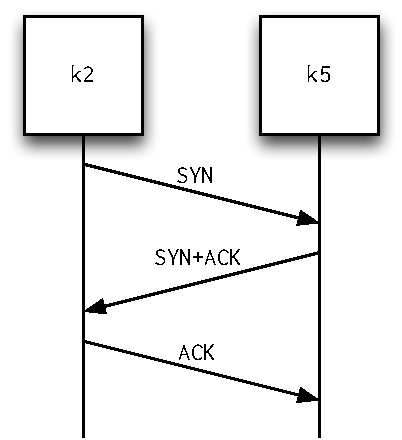
\includegraphics[width=5cm]{figury/stanowe/handshake-od-k2.pdf}}
  \qquad\qquad\qquad
  \subfloat[][]{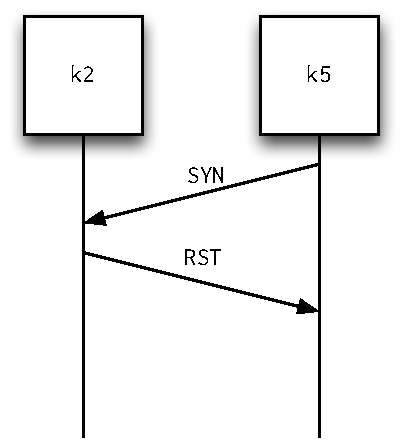
\includegraphics[width=5cm]{figury/stanowe/handshake-od-k5.pdf}}
  \caption{Wymiana komunikatów podczas \emph{handshake} przy nawiązywaniu połączenia przez maszyny po obu stronach zapory.}
  \label{fig:stanowe:handshake}
\end{figure}


\subsubsection{Wykonanie}

Wyczyszczono wszystkie reguły zapory \ipfw:

\begin{lstlisting}
k2% ipfw -q -f flush
\end{lstlisting}

Za pomocą programu \nc{} na maszynie \kpiec{} nasłuchiwano połączeń na porcie
\pos. Połączenie nawiązano z maszyny \kdwa{}. Potwierdzono, że nie ma problemu z
nawiązaniem takiego połączenia. Zbadano połączenie odwrotne. Na maszynie \kdwa{}
nasłuchiwano na porcie 6666, a nadawono z portu 80. Udało się nawiązać
połączenie.

% Nierówne są, coś ma dodatkowy margines. Jeśli suma szerokości
% minipage'y to 1\linewidth, to zajmują więcej niż linewidth.
\begin{minipage}[b]{0.4\linewidth}
\begin{lstlisting}
k2$ netcat k5 80
test
^D

k2$ netcat -l 6666
test test
k2$
\end{lstlisting}
\end{minipage}
\begin{minipage}[b]{0.12\linewidth}
  \hfill\vspace{1cm}
\end{minipage}
\begin{minipage}[b]{0.4\linewidth}
\begin{lstlisting}
k5$ netcat -l 80
test


k5$ netcat -p 80 k2 6666
test test
^D
\end{lstlisting}
\end{minipage}

Po nawiązaniu udanym nawiązaniu połączeń z obu stron rozpoczęto konfigurację
zapory. Dobrą praktyką jest rozpoczynanie konfiguracji zapory od zablokowania
całego ruchu. Niestety do prawidłowego działania maszyny niezbędne jest wiele
połączeń: \ssh{}, \texttt{LDAP}, \texttt{NAS}. Zdecydowano się na
\emph{blacklisting}. Praktyka ta polega na domyślnym przyjmowaniu wszystkich
połączeń. Jednocześnie część połączeń, zdefiniowanych na \emph{czarnej liście}
jest odrzucana. Przy tym trybie deklarowania reguł łatwo jest nieumyślnie
przeoczyć połączenie, które powinno być zablokowane i narazić sieć na atak lub
nadużycia. Dlatego nie jest to zalecany tryb konfiguracji zapory
\cite{bsd:firewall}.

W przypadku zapory stanowej można bardzo łatwo wprowadzić politykę odwrotną,
tzw. politykę białej listy. Domyślnie wszystkie pakiety przychodzące byłyby
odrzucane, natomiast pakiety wychodzące tworzyłyby nowe dynamiczne reguły.
Reguły te pozwalałyby odbiorcom pakietów na dostarczenie odpowiedzi.

Taka prosta konfiguracja zakłada, że użytkownicy w sieci chronionej firewallem
mogą być obdarzeni pełnym zaufaniem i nieograniczonym dostępem do Internetu.


\subsubsection{Konfiguracja zapory}

Na maszynie \kdwa{} zostały skonfigurowane następujące reguły zapory:

\begin{lstlisting}
00100 check-state
00150 allow tcp from any to any dst-port 80 out keep-state
00250 deny log logamount 100 ip from any to any src-port 80 in
65535 allow ip from any to any
\end{lstlisting}

Reguły \texttt{150} i \texttt{250} są podobne do tych omawianych w sekcji
\ref{sec:bezstanowe}. Zezwolono na połączenia \tcp{} wychodzące, których celem
jest dowolny adres i port \pos. Zabroniono natomiast wszystkich połączeń
przychodzących, których źródłem jest port \pos.

Dodatkowo dyrektywa \texttt{keep-state} w regule \texttt{150} instruuje zaporę,
aby dodała nowe reguły dynamiczne odpowiadające adresom i portom wykorzystanym
do połączenia \cite{bsd:firewall}. Dynamiczna reguła zostanie utworzona tylko
kiedy reguła zostanie dopasowana do połączenia.

Gdyby były to jedyne reguły, nawiązanie połączenia \tcp{} przez maszynę \kdwa{}
byłoby niemożliwe. Dzieje się tak ponieważ samo utworzenie dynamicznych reguł
nie wystarczy. Należy jeszcze dodać dyrektywę, która instruuje zaporę by
sprawdziła czy aktualny pakiet pasuje do którejś z dynamicznych reguł.

Zależało nam, aby dynamiczne reguły były sprawdzone zanim odrzucimy pakiet, z
reguły \texttt{250}. Dodano więc dyrektywę \texttt{check-state} jako regułę
\texttt{100} -- pierwszą w zestawie reguł naszej zapory.

Przy takiej konfiguracji zapora najpierw sprawdzi, czy przychodzący pakiet
pasuje do reguł dynamicznych. Jeżeli tak, zostanie on zaakceptowany. Jeżeli nie,
zapora będzie kontynuwać działanie próbując dopasować pakiet do reguł
statycznych.


\subsubsection{Testy}

Przeprowadzono testy analogiczne do tych z początku ćwiczenia.

\begin{minipage}[b]{0.4\linewidth}
\begin{lstlisting}[caption={\kdwa{}}]
k2$ netcat k5 80
test
^D

k2$ netcat -l 6666
k2$
\end{lstlisting}
\end{minipage}
\begin{minipage}[b]{0.12\linewidth}
  \hfill\vspace{1cm}
\end{minipage}
\begin{minipage}[b]{0.4\linewidth}
\begin{lstlisting}[caption={\kpiec{}}]
k5$ netcat -l 80
test
k5$ netcat -p 80 k2 6666
test test
TEST
^D
\end{lstlisting}
\end{minipage}

Można zauważyć na listingach, że osiągnęto zamierzony efekt. W drugim przypadku
testowym nie udało się nawiązać połączenia i przesłać danych do maszyny \kdwa.



\section{Wnioski}
% TODO GOOBY PLS
System FreeBSD  wyposażony jest w dojrzałe i dobrze udokumentowane narzędzia do konfiguracji zapór sieciowych.

Konfiguracja nawet prostej zapory na zasadzie białej listy w złożonym systemie może wymagać dużo pracy - należy zebrać wszystkie usługi z których korzysta system.
Takie rozwiązanie jest jednak dużo bezpieczniejsze od rozwiązania opartego o czarną listę.

Konfiguracja zapory opartej o białą listę jest tym trudniejsza, jeśli nie ma fizycznego dostępu do komputera który konfigurujemy.
Łatwo można doprowadzić komputer do stanu, w którym z różnych powodów nie można się na niego zalogować.
Zapora musi być budowana tak, aby po dodaniu każdej kolejnej reguły ciągle pozwalała na wszystkie połączenia wymagane do pracy zdalnej.
Może to wymagać dodawania reguł w innej kolejności, niż będą stosowane przez zaporę, dlatego \ipfw{} pozwala na podanie numeru dodawanej reguły.

Zapory z regułami stanowymi znacząco ułatwiają proste konfiguracje, w których można zaufać użytkownikom wewnątrz chronionego fragmentu sieci.



%\section{Bibliografia}
\begin{thebibliography}{99}
\bibitem{wstep:stevens}
    \emph{TCP/IP Illustrated --- 2nd ed.}; Kevin R. Fall, W. Richard Stevens; Pearson Education, Inc.\\
    Rozdział 7.2
\bibitem{bsd:firewall}
    \emph{FreeBSD Handbook}\\
    Rozdział 31 Firewalls
% Nah mon. Cytujemy źródła Wikipedii, nie Wikipedię.
% \bibitem{wiki:firewall}
%     \emph{Wikipedia}\\
%     Firewall (computing)
\end{thebibliography}



\end{document}
